\documentclass[twoside]{book}

% Packages required by doxygen
\usepackage{fixltx2e}
\usepackage{calc}
\usepackage{doxygen}
\usepackage[export]{adjustbox} % also loads graphicx
\usepackage{graphicx}
\usepackage[utf8]{inputenc}
\usepackage{makeidx}
\usepackage{multicol}
\usepackage{multirow}
\PassOptionsToPackage{warn}{textcomp}
\usepackage{textcomp}
\usepackage[nointegrals]{wasysym}
\usepackage[table]{xcolor}

% Font selection
\usepackage[T1]{fontenc}
\usepackage[scaled=.90]{helvet}
\usepackage{courier}
\usepackage{amssymb}
\usepackage{sectsty}
\renewcommand{\familydefault}{\sfdefault}
\allsectionsfont{%
  \fontseries{bc}\selectfont%
  \color{darkgray}%
}
\renewcommand{\DoxyLabelFont}{%
  \fontseries{bc}\selectfont%
  \color{darkgray}%
}
\newcommand{\+}{\discretionary{\mbox{\scriptsize$\hookleftarrow$}}{}{}}

% Page & text layout
\usepackage{geometry}
\geometry{%
  a4paper,%
  top=2.5cm,%
  bottom=2.5cm,%
  left=2.5cm,%
  right=2.5cm%
}
\tolerance=750
\hfuzz=15pt
\hbadness=750
\setlength{\emergencystretch}{15pt}
\setlength{\parindent}{0cm}
\setlength{\parskip}{3ex plus 2ex minus 2ex}
\makeatletter
\renewcommand{\paragraph}{%
  \@startsection{paragraph}{4}{0ex}{-1.0ex}{1.0ex}{%
    \normalfont\normalsize\bfseries\SS@parafont%
  }%
}
\renewcommand{\subparagraph}{%
  \@startsection{subparagraph}{5}{0ex}{-1.0ex}{1.0ex}{%
    \normalfont\normalsize\bfseries\SS@subparafont%
  }%
}
\makeatother

% Headers & footers
\usepackage{fancyhdr}
\pagestyle{fancyplain}
\fancyhead[LE]{\fancyplain{}{\bfseries\thepage}}
\fancyhead[CE]{\fancyplain{}{}}
\fancyhead[RE]{\fancyplain{}{\bfseries\leftmark}}
\fancyhead[LO]{\fancyplain{}{\bfseries\rightmark}}
\fancyhead[CO]{\fancyplain{}{}}
\fancyhead[RO]{\fancyplain{}{\bfseries\thepage}}
\fancyfoot[LE]{\fancyplain{}{}}
\fancyfoot[CE]{\fancyplain{}{}}
\fancyfoot[RE]{\fancyplain{}{\bfseries\scriptsize Generated by Doxygen }}
\fancyfoot[LO]{\fancyplain{}{\bfseries\scriptsize Generated by Doxygen }}
\fancyfoot[CO]{\fancyplain{}{}}
\fancyfoot[RO]{\fancyplain{}{}}
\renewcommand{\footrulewidth}{0.4pt}
\renewcommand{\chaptermark}[1]{%
  \markboth{#1}{}%
}
\renewcommand{\sectionmark}[1]{%
  \markright{\thesection\ #1}%
}

% Indices & bibliography
\usepackage{natbib}
\usepackage[titles]{tocloft}
\setcounter{tocdepth}{3}
\setcounter{secnumdepth}{5}
\makeindex

% Hyperlinks (required, but should be loaded last)
\usepackage{ifpdf}
\ifpdf
  \usepackage[pdftex,pagebackref=true]{hyperref}
\else
  \usepackage[ps2pdf,pagebackref=true]{hyperref}
\fi
\hypersetup{%
  colorlinks=true,%
  linkcolor=blue,%
  citecolor=blue,%
  unicode%
}

% Custom commands
\newcommand{\clearemptydoublepage}{%
  \newpage{\pagestyle{empty}\cleardoublepage}%
}

\usepackage{caption}
\captionsetup{labelsep=space,justification=centering,font={bf},singlelinecheck=off,skip=4pt,position=top}

%===== C O N T E N T S =====

\begin{document}

% Titlepage & ToC
\hypersetup{pageanchor=false,
             bookmarksnumbered=true,
             pdfencoding=unicode
            }
\pagenumbering{alph}
\begin{titlepage}
\vspace*{7cm}
\begin{center}%
{\Large Wave\+Simulator }\\
\vspace*{1cm}
{\large Generated by Doxygen 1.8.13}\\
\end{center}
\end{titlepage}
\clearemptydoublepage
\pagenumbering{roman}
\tableofcontents
\clearemptydoublepage
\pagenumbering{arabic}
\hypersetup{pageanchor=true}

%--- Begin generated contents ---
\chapter{Hierarchical Index}
\section{Class Hierarchy}
This inheritance list is sorted roughly, but not completely, alphabetically\+:\begin{DoxyCompactList}
\item \contentsline{section}{Solver.\+C\+P\+P\+Simulator}{\pageref{classSolver_1_1CPPSimulator}}{}
\item \contentsline{section}{Float1D}{\pageref{classFloat1D}}{}
\item \contentsline{section}{Float2D}{\pageref{classFloat2D}}{}
\item \contentsline{section}{Solver.\+Helper}{\pageref{classSolver_1_1Helper}}{}
\item On\+Double\+Tap\+Listener\begin{DoxyCompactList}
\item \contentsline{section}{Interface.\+Wave\+View\+Touch\+Listener}{\pageref{classInterface_1_1WaveViewTouchListener}}{}
\end{DoxyCompactList}
\item On\+Gesture\+Listener\begin{DoxyCompactList}
\item \contentsline{section}{Interface.\+Wave\+View\+Touch\+Listener}{\pageref{classInterface_1_1WaveViewTouchListener}}{}
\end{DoxyCompactList}
\item On\+Touch\+Listener\begin{DoxyCompactList}
\item \contentsline{section}{Interface.\+Wave\+View\+Touch\+Listener}{\pageref{classInterface_1_1WaveViewTouchListener}}{}
\end{DoxyCompactList}
\item \contentsline{section}{Solver.\+Simulation\+Runner}{\pageref{classSolver_1_1SimulationRunner}}{}
\item \contentsline{section}{S\+W\+E\+\_\+\+Block}{\pageref{classSWE__Block}}{}
\begin{DoxyCompactList}
\item \contentsline{section}{S\+W\+E\+\_\+\+Wave\+Propagation\+Block}{\pageref{classSWE__WavePropagationBlock}}{}
\end{DoxyCompactList}
\item \contentsline{section}{S\+W\+E\+\_\+\+Block1D}{\pageref{structSWE__Block1D}}{}
\item \contentsline{section}{S\+W\+E\+\_\+\+Scenario}{\pageref{classSWE__Scenario}}{}
\begin{DoxyCompactList}
\item \contentsline{section}{S\+W\+E\+\_\+\+Flat\+Scenario}{\pageref{classSWE__FlatScenario}}{}
\end{DoxyCompactList}
\item \contentsline{section}{Wave\+Propagation}{\pageref{classWavePropagation}}{}
\item \contentsline{section}{solver\+:\+:Wave\+Propagation$<$ T $>$}{\pageref{classsolver_1_1WavePropagation}}{}
\item App\+Compat\+Activity\begin{DoxyCompactList}
\item \contentsline{section}{Interface.\+Main\+Activity}{\pageref{classInterface_1_1MainActivity}}{}
\end{DoxyCompactList}
\item View\begin{DoxyCompactList}
\item \contentsline{section}{Interface.\+Wave\+View}{\pageref{classInterface_1_1WaveView}}{}
\end{DoxyCompactList}
\end{DoxyCompactList}

\chapter{Class Index}
\section{Class List}
Here are the classes, structs, unions and interfaces with brief descriptions\+:\begin{DoxyCompactList}
\item\contentsline{section}{\hyperlink{classSolver_1_1CPPSimulator}{Solver.\+C\+P\+P\+Simulator} }{\pageref{classSolver_1_1CPPSimulator}}{}
\item\contentsline{section}{\hyperlink{classSolver_1_1Helper}{Solver.\+Helper} }{\pageref{classSolver_1_1Helper}}{}
\item\contentsline{section}{\hyperlink{classwavesimulator_1_1MainActivity}{wavesimulator.\+Main\+Activity} }{\pageref{classwavesimulator_1_1MainActivity}}{}
\item\contentsline{section}{\hyperlink{classSolver_1_1SimulationRunner}{Solver.\+Simulation\+Runner} }{\pageref{classSolver_1_1SimulationRunner}}{}
\item\contentsline{section}{\hyperlink{classwavesimulator_1_1WaveView}{wavesimulator.\+Wave\+View} }{\pageref{classwavesimulator_1_1WaveView}}{}
\item\contentsline{section}{\hyperlink{classwavesimulator_1_1WaveViewTouchListener}{wavesimulator.\+Wave\+View\+Touch\+Listener} }{\pageref{classwavesimulator_1_1WaveViewTouchListener}}{}
\end{DoxyCompactList}

\chapter{Class Documentation}
\hypertarget{classSolver_1_1CPPSimulator}{}\section{Solver.\+C\+P\+P\+Simulator Class Reference}
\label{classSolver_1_1CPPSimulator}\index{Solver.\+C\+P\+P\+Simulator@{Solver.\+C\+P\+P\+Simulator}}


Collaboration diagram for Solver.\+C\+P\+P\+Simulator\+:

\hypertarget{classSolver_1_1Helper}{}\section{Solver.\+Helper Class Reference}
\label{classSolver_1_1Helper}\index{Solver.\+Helper@{Solver.\+Helper}}


This class contains a helper method that maps a number of the x domain onto the y domain via linearisation;.  


\subsection*{Static Public Member Functions}
\begin{DoxyCompactItemize}
\item 
static float \hyperlink{classSolver_1_1Helper_ab4e2ecd76f5062902111a42657f748af}{linear\+\_\+map} (float x1, float y1, float x2, float y2, float number)
\end{DoxyCompactItemize}


\subsection{Detailed Description}
This class contains a helper method that maps a number of the x domain onto the y domain via linearisation;. 

Definition at line 3 of file Helper.\+java.



\subsection{Member Function Documentation}
\index{Solver\+::\+Helper@{Solver\+::\+Helper}!linear\+\_\+map@{linear\+\_\+map}}
\index{linear\+\_\+map@{linear\+\_\+map}!Solver\+::\+Helper@{Solver\+::\+Helper}}
\subsubsection[{\texorpdfstring{linear\+\_\+map(float x1, float y1, float x2, float y2, float number)}{linear_map(float x1, float y1, float x2, float y2, float number)}}]{\setlength{\rightskip}{0pt plus 5cm}static float Solver.\+Helper.\+linear\+\_\+map (
\begin{DoxyParamCaption}
\item[{float}]{x1, }
\item[{float}]{y1, }
\item[{float}]{x2, }
\item[{float}]{y2, }
\item[{float}]{number}
\end{DoxyParamCaption}
)\hspace{0.3cm}{\ttfamily [inline]}, {\ttfamily [static]}}\hypertarget{classSolver_1_1Helper_ab4e2ecd76f5062902111a42657f748af}{}\label{classSolver_1_1Helper_ab4e2ecd76f5062902111a42657f748af}


Definition at line 5 of file Helper.\+java.



The documentation for this class was generated from the following file\+:\begin{DoxyCompactItemize}
\item 
app/src/main/java/\+Solver/\hyperlink{Helper_8java}{Helper.\+java}\end{DoxyCompactItemize}

\hypertarget{classwavesimulator_1_1MainActivity}{}\section{wavesimulator.\+Main\+Activity Class Reference}
\label{classwavesimulator_1_1MainActivity}\index{wavesimulator.\+Main\+Activity@{wavesimulator.\+Main\+Activity}}


This class handles the main-\/\+Activities.  




Inheritance diagram for wavesimulator.\+Main\+Activity\+:\nopagebreak
\begin{figure}[H]
\begin{center}
\leavevmode
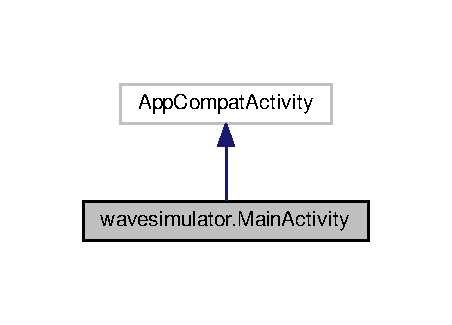
\includegraphics[width=217pt]{classwavesimulator_1_1MainActivity__inherit__graph}
\end{center}
\end{figure}


Collaboration diagram for wavesimulator.\+Main\+Activity\+:\nopagebreak
\begin{figure}[H]
\begin{center}
\leavevmode
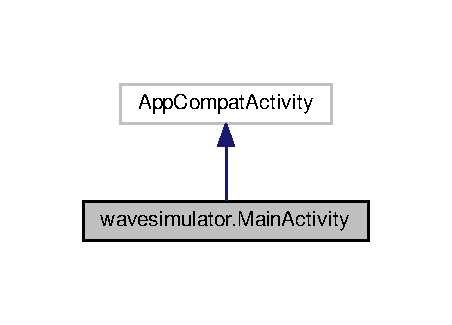
\includegraphics[width=217pt]{classwavesimulator_1_1MainActivity__coll__graph}
\end{center}
\end{figure}
\subsection*{Public Member Functions}
\begin{DoxyCompactItemize}
\item 
boolean \hyperlink{classwavesimulator_1_1MainActivity_aec42f57753b20a3200ff2d6faefbbfd6}{on\+Create\+Options\+Menu} (Menu menu)
\item 
boolean \hyperlink{classwavesimulator_1_1MainActivity_ac1e77788cf8d6eee4b48ccfec120b414}{on\+Options\+Item\+Selected} (Menu\+Item item)
\begin{DoxyCompactList}\small\item\em gets called if a menu item is selected \end{DoxyCompactList}\item 
void \hyperlink{classwavesimulator_1_1MainActivity_ad4717a53e98a2eeb4be677b754169d6d}{Wave\+Height\+Seek\+Bar\+Changed} ()
\begin{DoxyCompactList}\small\item\em gets called when the user uses the waveheight seekbar \end{DoxyCompactList}\item 
float \hyperlink{classwavesimulator_1_1MainActivity_a7b2a54961e6db516c70463c0a5a12e21}{get\+Wave\+Height\+Value} ()
\item 
void \hyperlink{classwavesimulator_1_1MainActivity_aa4b02a928bcf917374e14fa2950f3659}{on\+Checked\+Switch} (Compound\+Button button\+View, boolean is\+Checked)
\begin{DoxyCompactList}\small\item\em gets called when the user uses the wall boundary switch \end{DoxyCompactList}\item 
\hyperlink{classwavesimulator_1_1WaveView}{Wave\+View} \hyperlink{classwavesimulator_1_1MainActivity_a6f24f2ef94993440a4e7c7df229a0e97}{get\+Wave\+View} ()
\end{DoxyCompactItemize}
\subsection*{Static Public Member Functions}
\begin{DoxyCompactItemize}
\item 
static \hyperlink{classSolver_1_1SimulationRunner}{Simulation\+Runner} \hyperlink{classwavesimulator_1_1MainActivity_a79c45b397d8e357efbf26d07822b93dc}{get\+Simulation\+Runner} ()
\end{DoxyCompactItemize}
\subsection*{Protected Member Functions}
\begin{DoxyCompactItemize}
\item 
void \hyperlink{classwavesimulator_1_1MainActivity_ac68987419bcdc1f93e4501a7642dbf04}{on\+Create} (Bundle saved\+Instance\+State)
\end{DoxyCompactItemize}


\subsection{Detailed Description}
This class handles the main-\/\+Activities. 

Definition at line 24 of file Main\+Activity.\+java.



\subsection{Member Function Documentation}
\index{wavesimulator\+::\+Main\+Activity@{wavesimulator\+::\+Main\+Activity}!get\+Simulation\+Runner@{get\+Simulation\+Runner}}
\index{get\+Simulation\+Runner@{get\+Simulation\+Runner}!wavesimulator\+::\+Main\+Activity@{wavesimulator\+::\+Main\+Activity}}
\subsubsection[{\texorpdfstring{get\+Simulation\+Runner()}{getSimulationRunner()}}]{\setlength{\rightskip}{0pt plus 5cm}static {\bf Simulation\+Runner} wavesimulator.\+Main\+Activity.\+get\+Simulation\+Runner (
\begin{DoxyParamCaption}
{}
\end{DoxyParamCaption}
)\hspace{0.3cm}{\ttfamily [inline]}, {\ttfamily [static]}}\hypertarget{classwavesimulator_1_1MainActivity_a79c45b397d8e357efbf26d07822b93dc}{}\label{classwavesimulator_1_1MainActivity_a79c45b397d8e357efbf26d07822b93dc}


Definition at line 177 of file Main\+Activity.\+java.

\index{wavesimulator\+::\+Main\+Activity@{wavesimulator\+::\+Main\+Activity}!get\+Wave\+Height\+Value@{get\+Wave\+Height\+Value}}
\index{get\+Wave\+Height\+Value@{get\+Wave\+Height\+Value}!wavesimulator\+::\+Main\+Activity@{wavesimulator\+::\+Main\+Activity}}
\subsubsection[{\texorpdfstring{get\+Wave\+Height\+Value()}{getWaveHeightValue()}}]{\setlength{\rightskip}{0pt plus 5cm}float wavesimulator.\+Main\+Activity.\+get\+Wave\+Height\+Value (
\begin{DoxyParamCaption}
{}
\end{DoxyParamCaption}
)\hspace{0.3cm}{\ttfamily [inline]}}\hypertarget{classwavesimulator_1_1MainActivity_a7b2a54961e6db516c70463c0a5a12e21}{}\label{classwavesimulator_1_1MainActivity_a7b2a54961e6db516c70463c0a5a12e21}
$<$ maps the seekbarvalue(0,100) to the waveheight(5,15) 

Definition at line 164 of file Main\+Activity.\+java.

\index{wavesimulator\+::\+Main\+Activity@{wavesimulator\+::\+Main\+Activity}!get\+Wave\+View@{get\+Wave\+View}}
\index{get\+Wave\+View@{get\+Wave\+View}!wavesimulator\+::\+Main\+Activity@{wavesimulator\+::\+Main\+Activity}}
\subsubsection[{\texorpdfstring{get\+Wave\+View()}{getWaveView()}}]{\setlength{\rightskip}{0pt plus 5cm}{\bf Wave\+View} wavesimulator.\+Main\+Activity.\+get\+Wave\+View (
\begin{DoxyParamCaption}
{}
\end{DoxyParamCaption}
)\hspace{0.3cm}{\ttfamily [inline]}}\hypertarget{classwavesimulator_1_1MainActivity_a6f24f2ef94993440a4e7c7df229a0e97}{}\label{classwavesimulator_1_1MainActivity_a6f24f2ef94993440a4e7c7df229a0e97}


Definition at line 173 of file Main\+Activity.\+java.

\index{wavesimulator\+::\+Main\+Activity@{wavesimulator\+::\+Main\+Activity}!on\+Checked\+Switch@{on\+Checked\+Switch}}
\index{on\+Checked\+Switch@{on\+Checked\+Switch}!wavesimulator\+::\+Main\+Activity@{wavesimulator\+::\+Main\+Activity}}
\subsubsection[{\texorpdfstring{on\+Checked\+Switch(\+Compound\+Button button\+View, boolean is\+Checked)}{onCheckedSwitch(CompoundButton buttonView, boolean isChecked)}}]{\setlength{\rightskip}{0pt plus 5cm}void wavesimulator.\+Main\+Activity.\+on\+Checked\+Switch (
\begin{DoxyParamCaption}
\item[{Compound\+Button}]{button\+View, }
\item[{boolean}]{is\+Checked}
\end{DoxyParamCaption}
)\hspace{0.3cm}{\ttfamily [inline]}}\hypertarget{classwavesimulator_1_1MainActivity_aa4b02a928bcf917374e14fa2950f3659}{}\label{classwavesimulator_1_1MainActivity_aa4b02a928bcf917374e14fa2950f3659}


gets called when the user uses the wall boundary switch 



Definition at line 169 of file Main\+Activity.\+java.

\index{wavesimulator\+::\+Main\+Activity@{wavesimulator\+::\+Main\+Activity}!on\+Create@{on\+Create}}
\index{on\+Create@{on\+Create}!wavesimulator\+::\+Main\+Activity@{wavesimulator\+::\+Main\+Activity}}
\subsubsection[{\texorpdfstring{on\+Create(\+Bundle saved\+Instance\+State)}{onCreate(Bundle savedInstanceState)}}]{\setlength{\rightskip}{0pt plus 5cm}void wavesimulator.\+Main\+Activity.\+on\+Create (
\begin{DoxyParamCaption}
\item[{Bundle}]{saved\+Instance\+State}
\end{DoxyParamCaption}
)\hspace{0.3cm}{\ttfamily [inline]}, {\ttfamily [protected]}}\hypertarget{classwavesimulator_1_1MainActivity_ac68987419bcdc1f93e4501a7642dbf04}{}\label{classwavesimulator_1_1MainActivity_ac68987419bcdc1f93e4501a7642dbf04}
$<$ Defines the on\+Click Listener for the switch

$<$ Defines Touchlistener of the Waveview

$<$ set Listener of the waveheight seekbar

$<$ add the toolbar to the main activity

$<$ create a new simulation runner or set the current activity in the existing one 

Definition at line 47 of file Main\+Activity.\+java.

\index{wavesimulator\+::\+Main\+Activity@{wavesimulator\+::\+Main\+Activity}!on\+Create\+Options\+Menu@{on\+Create\+Options\+Menu}}
\index{on\+Create\+Options\+Menu@{on\+Create\+Options\+Menu}!wavesimulator\+::\+Main\+Activity@{wavesimulator\+::\+Main\+Activity}}
\subsubsection[{\texorpdfstring{on\+Create\+Options\+Menu(\+Menu menu)}{onCreateOptionsMenu(Menu menu)}}]{\setlength{\rightskip}{0pt plus 5cm}boolean wavesimulator.\+Main\+Activity.\+on\+Create\+Options\+Menu (
\begin{DoxyParamCaption}
\item[{Menu}]{menu}
\end{DoxyParamCaption}
)\hspace{0.3cm}{\ttfamily [inline]}}\hypertarget{classwavesimulator_1_1MainActivity_aec42f57753b20a3200ff2d6faefbbfd6}{}\label{classwavesimulator_1_1MainActivity_aec42f57753b20a3200ff2d6faefbbfd6}
$<$ sets the custom menu to the actionbar 

Definition at line 94 of file Main\+Activity.\+java.

\index{wavesimulator\+::\+Main\+Activity@{wavesimulator\+::\+Main\+Activity}!on\+Options\+Item\+Selected@{on\+Options\+Item\+Selected}}
\index{on\+Options\+Item\+Selected@{on\+Options\+Item\+Selected}!wavesimulator\+::\+Main\+Activity@{wavesimulator\+::\+Main\+Activity}}
\subsubsection[{\texorpdfstring{on\+Options\+Item\+Selected(\+Menu\+Item item)}{onOptionsItemSelected(MenuItem item)}}]{\setlength{\rightskip}{0pt plus 5cm}boolean wavesimulator.\+Main\+Activity.\+on\+Options\+Item\+Selected (
\begin{DoxyParamCaption}
\item[{Menu\+Item}]{item}
\end{DoxyParamCaption}
)\hspace{0.3cm}{\ttfamily [inline]}}\hypertarget{classwavesimulator_1_1MainActivity_ac1e77788cf8d6eee4b48ccfec120b414}{}\label{classwavesimulator_1_1MainActivity_ac1e77788cf8d6eee4b48ccfec120b414}


gets called if a menu item is selected 

$<$ reset is selected

$<$ reloads the Simulation;

$<$ resetboundary Switch

$<$ reset wave is selected

$<$ brush mode is selected

\begin{quote}
if its already in the draw mode, disable draw mode \end{quote}


\begin{quote}
if not, disable erase mode and enable drawmode \end{quote}


$<$ erase mode is selected

\begin{quote}
if its already in the erase mode, disable erase mode \end{quote}


\begin{quote}
if not, disable draw mode and enable erase mode \end{quote}


\begin{quote}
show snackbar which explains current action \end{quote}


Definition at line 102 of file Main\+Activity.\+java.

\index{wavesimulator\+::\+Main\+Activity@{wavesimulator\+::\+Main\+Activity}!Wave\+Height\+Seek\+Bar\+Changed@{Wave\+Height\+Seek\+Bar\+Changed}}
\index{Wave\+Height\+Seek\+Bar\+Changed@{Wave\+Height\+Seek\+Bar\+Changed}!wavesimulator\+::\+Main\+Activity@{wavesimulator\+::\+Main\+Activity}}
\subsubsection[{\texorpdfstring{Wave\+Height\+Seek\+Bar\+Changed()}{WaveHeightSeekBarChanged()}}]{\setlength{\rightskip}{0pt plus 5cm}void wavesimulator.\+Main\+Activity.\+Wave\+Height\+Seek\+Bar\+Changed (
\begin{DoxyParamCaption}
{}
\end{DoxyParamCaption}
)\hspace{0.3cm}{\ttfamily [inline]}}\hypertarget{classwavesimulator_1_1MainActivity_ad4717a53e98a2eeb4be677b754169d6d}{}\label{classwavesimulator_1_1MainActivity_ad4717a53e98a2eeb4be677b754169d6d}


gets called when the user uses the waveheight seekbar 

$<$ inform user about current waveheight 

Definition at line 157 of file Main\+Activity.\+java.



The documentation for this class was generated from the following file\+:\begin{DoxyCompactItemize}
\item 
app/src/main/java/wavesimulator/\hyperlink{MainActivity_8java}{Main\+Activity.\+java}\end{DoxyCompactItemize}

\hypertarget{classSolver_1_1SimulationRunner}{}\section{Solver.\+Simulation\+Runner Class Reference}
\label{classSolver_1_1SimulationRunner}\index{Solver.\+Simulation\+Runner@{Solver.\+Simulation\+Runner}}
\subsection*{Public Member Functions}
\begin{DoxyCompactItemize}
\item 
\mbox{\Hypertarget{classSolver_1_1SimulationRunner_a58f6020d625c60b8a04329eced280ca9}\label{classSolver_1_1SimulationRunner_a58f6020d625c60b8a04329eced280ca9}} 
{\bfseries Simulation\+Runner} (\hyperlink{classwavesimulator_1_1MainActivity}{Main\+Activity} current\+Activity)
\item 
\mbox{\Hypertarget{classSolver_1_1SimulationRunner_ab34c984e38253223884911c042175426}\label{classSolver_1_1SimulationRunner_ab34c984e38253223884911c042175426}} 
void {\bfseries start} ()
\item 
\mbox{\Hypertarget{classSolver_1_1SimulationRunner_ab44a9a2edd9aec16fe26bb05fa0f1115}\label{classSolver_1_1SimulationRunner_ab44a9a2edd9aec16fe26bb05fa0f1115}} 
void {\bfseries change\+Activity} (\hyperlink{classwavesimulator_1_1MainActivity}{Main\+Activity} a)
\item 
\mbox{\Hypertarget{classSolver_1_1SimulationRunner_a9b9b7707ac2d73e32cc86d3d0a609dde}\label{classSolver_1_1SimulationRunner_a9b9b7707ac2d73e32cc86d3d0a609dde}} 
void {\bfseries stop} ()
\item 
\mbox{\Hypertarget{classSolver_1_1SimulationRunner_a6b7b251488a9854ee2221e3fd37e4c26}\label{classSolver_1_1SimulationRunner_a6b7b251488a9854ee2221e3fd37e4c26}} 
boolean {\bfseries is\+Started} ()
\end{DoxyCompactItemize}


The documentation for this class was generated from the following file\+:\begin{DoxyCompactItemize}
\item 
app/src/main/java/\+Solver/Simulation\+Runner.\+java\end{DoxyCompactItemize}

\hypertarget{classwavesimulator_1_1WaveView}{}\section{wavesimulator.\+Wave\+View Class Reference}
\label{classwavesimulator_1_1WaveView}\index{wavesimulator.\+Wave\+View@{wavesimulator.\+Wave\+View}}


Inheritance diagram for wavesimulator.\+Wave\+View\+:
% FIG 0


Collaboration diagram for wavesimulator.\+Wave\+View\+:
% FIG 1
\subsection*{Public Member Functions}
\begin{DoxyCompactItemize}
\item 
\mbox{\Hypertarget{classwavesimulator_1_1WaveView_a9ec88e17333db01de8637efedf66fa1b}\label{classwavesimulator_1_1WaveView_a9ec88e17333db01de8637efedf66fa1b}} 
{\bfseries Wave\+View} (Context context, Attribute\+Set attrs)
\item 
\mbox{\Hypertarget{classwavesimulator_1_1WaveView_a2c9aa15893e998681246c9c9ae0de77f}\label{classwavesimulator_1_1WaveView_a2c9aa15893e998681246c9c9ae0de77f}} 
void {\bfseries on\+Draw} (Canvas canvas)
\end{DoxyCompactItemize}
\subsection*{Protected Member Functions}
\begin{DoxyCompactItemize}
\item 
\mbox{\Hypertarget{classwavesimulator_1_1WaveView_ad7e6b1acf6ec2359283332d6dd86b901}\label{classwavesimulator_1_1WaveView_ad7e6b1acf6ec2359283332d6dd86b901}} 
void {\bfseries on\+Size\+Changed} (int w, int h, int old\+\_\+w, int old\+\_\+h)
\end{DoxyCompactItemize}


The documentation for this class was generated from the following file\+:\begin{DoxyCompactItemize}
\item 
app/src/main/java/wavesimulator/Wave\+View.\+java\end{DoxyCompactItemize}

\hypertarget{classwavesimulator_1_1WaveViewTouchListener}{}\section{wavesimulator.\+Wave\+View\+Touch\+Listener Class Reference}
\label{classwavesimulator_1_1WaveViewTouchListener}\index{wavesimulator.\+Wave\+View\+Touch\+Listener@{wavesimulator.\+Wave\+View\+Touch\+Listener}}


Inheritance diagram for wavesimulator.\+Wave\+View\+Touch\+Listener\+:
% FIG 0


Collaboration diagram for wavesimulator.\+Wave\+View\+Touch\+Listener\+:
% FIG 1
\subsection*{Public Member Functions}
\begin{DoxyCompactItemize}
\item 
\mbox{\Hypertarget{classwavesimulator_1_1WaveViewTouchListener_a325c79c04591b29d1ccc2f17538f1b4e}\label{classwavesimulator_1_1WaveViewTouchListener_a325c79c04591b29d1ccc2f17538f1b4e}} 
boolean {\bfseries on\+Touch} (View view, Motion\+Event motion\+Event)
\item 
\mbox{\Hypertarget{classwavesimulator_1_1WaveViewTouchListener_a812d58658cd4766b77acc6805c11bd5e}\label{classwavesimulator_1_1WaveViewTouchListener_a812d58658cd4766b77acc6805c11bd5e}} 
boolean {\bfseries on\+Single\+Tap\+Confirmed} (Motion\+Event motion\+Event)
\item 
\mbox{\Hypertarget{classwavesimulator_1_1WaveViewTouchListener_a9dc7880808de5d6211b235eea093010b}\label{classwavesimulator_1_1WaveViewTouchListener_a9dc7880808de5d6211b235eea093010b}} 
boolean {\bfseries on\+Double\+Tap} (Motion\+Event motion\+Event)
\item 
\mbox{\Hypertarget{classwavesimulator_1_1WaveViewTouchListener_a8fe377045999aa7d7e0c177602294a77}\label{classwavesimulator_1_1WaveViewTouchListener_a8fe377045999aa7d7e0c177602294a77}} 
boolean {\bfseries on\+Down} (Motion\+Event motion\+Event)
\item 
\mbox{\Hypertarget{classwavesimulator_1_1WaveViewTouchListener_a27e41c2afd3355b733980f0a1b3cc443}\label{classwavesimulator_1_1WaveViewTouchListener_a27e41c2afd3355b733980f0a1b3cc443}} 
void {\bfseries on\+Show\+Press} (Motion\+Event motion\+Event)
\item 
\mbox{\Hypertarget{classwavesimulator_1_1WaveViewTouchListener_a65b57a542917ca9748b4b1a61a1dfea3}\label{classwavesimulator_1_1WaveViewTouchListener_a65b57a542917ca9748b4b1a61a1dfea3}} 
boolean {\bfseries on\+Single\+Tap\+Up} (Motion\+Event motion\+Event)
\item 
\mbox{\Hypertarget{classwavesimulator_1_1WaveViewTouchListener_aca5036fc983c0688503c69c153c057f0}\label{classwavesimulator_1_1WaveViewTouchListener_aca5036fc983c0688503c69c153c057f0}} 
boolean {\bfseries on\+Double\+Tap\+Event} (Motion\+Event motion\+Event)
\item 
\mbox{\Hypertarget{classwavesimulator_1_1WaveViewTouchListener_ab9902752f747fee07f7ebba8f759e6ad}\label{classwavesimulator_1_1WaveViewTouchListener_ab9902752f747fee07f7ebba8f759e6ad}} 
boolean {\bfseries on\+Scroll} (Motion\+Event motion\+Event, Motion\+Event motion\+Event1, float v, float v1)
\item 
\mbox{\Hypertarget{classwavesimulator_1_1WaveViewTouchListener_a38c5a9641b2585940c53e9be126675fe}\label{classwavesimulator_1_1WaveViewTouchListener_a38c5a9641b2585940c53e9be126675fe}} 
void {\bfseries on\+Long\+Press} (Motion\+Event motion\+Event)
\item 
\mbox{\Hypertarget{classwavesimulator_1_1WaveViewTouchListener_ab5306d4dc5257a10a1494f8abefd102d}\label{classwavesimulator_1_1WaveViewTouchListener_ab5306d4dc5257a10a1494f8abefd102d}} 
boolean {\bfseries on\+Fling} (Motion\+Event motion\+Event, Motion\+Event motion\+Event1, float v, float v1)
\end{DoxyCompactItemize}
\subsection*{Public Attributes}
\begin{DoxyCompactItemize}
\item 
\mbox{\Hypertarget{classwavesimulator_1_1WaveViewTouchListener_a7ca3435bb1c387559ca1251e82fdf8a3}\label{classwavesimulator_1_1WaveViewTouchListener_a7ca3435bb1c387559ca1251e82fdf8a3}} 
int {\bfseries drawingmode}
\end{DoxyCompactItemize}
\subsection*{Static Public Attributes}
\begin{DoxyCompactItemize}
\item 
\mbox{\Hypertarget{classwavesimulator_1_1WaveViewTouchListener_a1d1220dca35324db02e3ac953db358ec}\label{classwavesimulator_1_1WaveViewTouchListener_a1d1220dca35324db02e3ac953db358ec}} 
static final int {\bfseries M\+O\+D\+E\+\_\+\+S\+I\+M\+U\+L\+A\+TE} = 0
\item 
\mbox{\Hypertarget{classwavesimulator_1_1WaveViewTouchListener_a43b9a5b29cc916665f118e4eb02ea0cd}\label{classwavesimulator_1_1WaveViewTouchListener_a43b9a5b29cc916665f118e4eb02ea0cd}} 
static final int {\bfseries M\+O\+D\+E\+\_\+\+D\+R\+AW} = 1
\item 
\mbox{\Hypertarget{classwavesimulator_1_1WaveViewTouchListener_a362216c62634446ed74cf63bb09dfcfa}\label{classwavesimulator_1_1WaveViewTouchListener_a362216c62634446ed74cf63bb09dfcfa}} 
static final int {\bfseries M\+O\+D\+E\+\_\+\+E\+R\+E\+A\+SE} = 2
\end{DoxyCompactItemize}


The documentation for this class was generated from the following file\+:\begin{DoxyCompactItemize}
\item 
app/src/main/java/wavesimulator/Wave\+View\+Touch\+Listener.\+java\end{DoxyCompactItemize}

%--- End generated contents ---

% Index
\backmatter
\newpage
\phantomsection
\clearemptydoublepage
\addcontentsline{toc}{chapter}{Index}
\printindex

\end{document}
